\section{Tiny Tapeout 1}
\label{sec:tinytapeout1}

The Tiny Tapeout project started as an experiment in fitting as many designs as possible into the \qty{10}{\milli\meter\squared} available on the Google lottery shuttles (Fig.~\ref{fig:500_designs_chain_TT01}) using the Efabless Caravel harness.
In order to prove the concept as rapidly as possible initial designs were based on a scan chain architecture to simplify testing.

Each Tiny Tapeout 1 design has eight inputs and eight outputs.
Clock and reset signals were optional and not treated specially. The chain was formed of scan flops~\cite{skywaterpdk}, a type of flip flop with a multiplexer integrated at its input. An example showing a two design scan chain is shown in Fig.~\ref{fig:simplified_view_2_designs}.

\begin{figure}[!t]
\centering
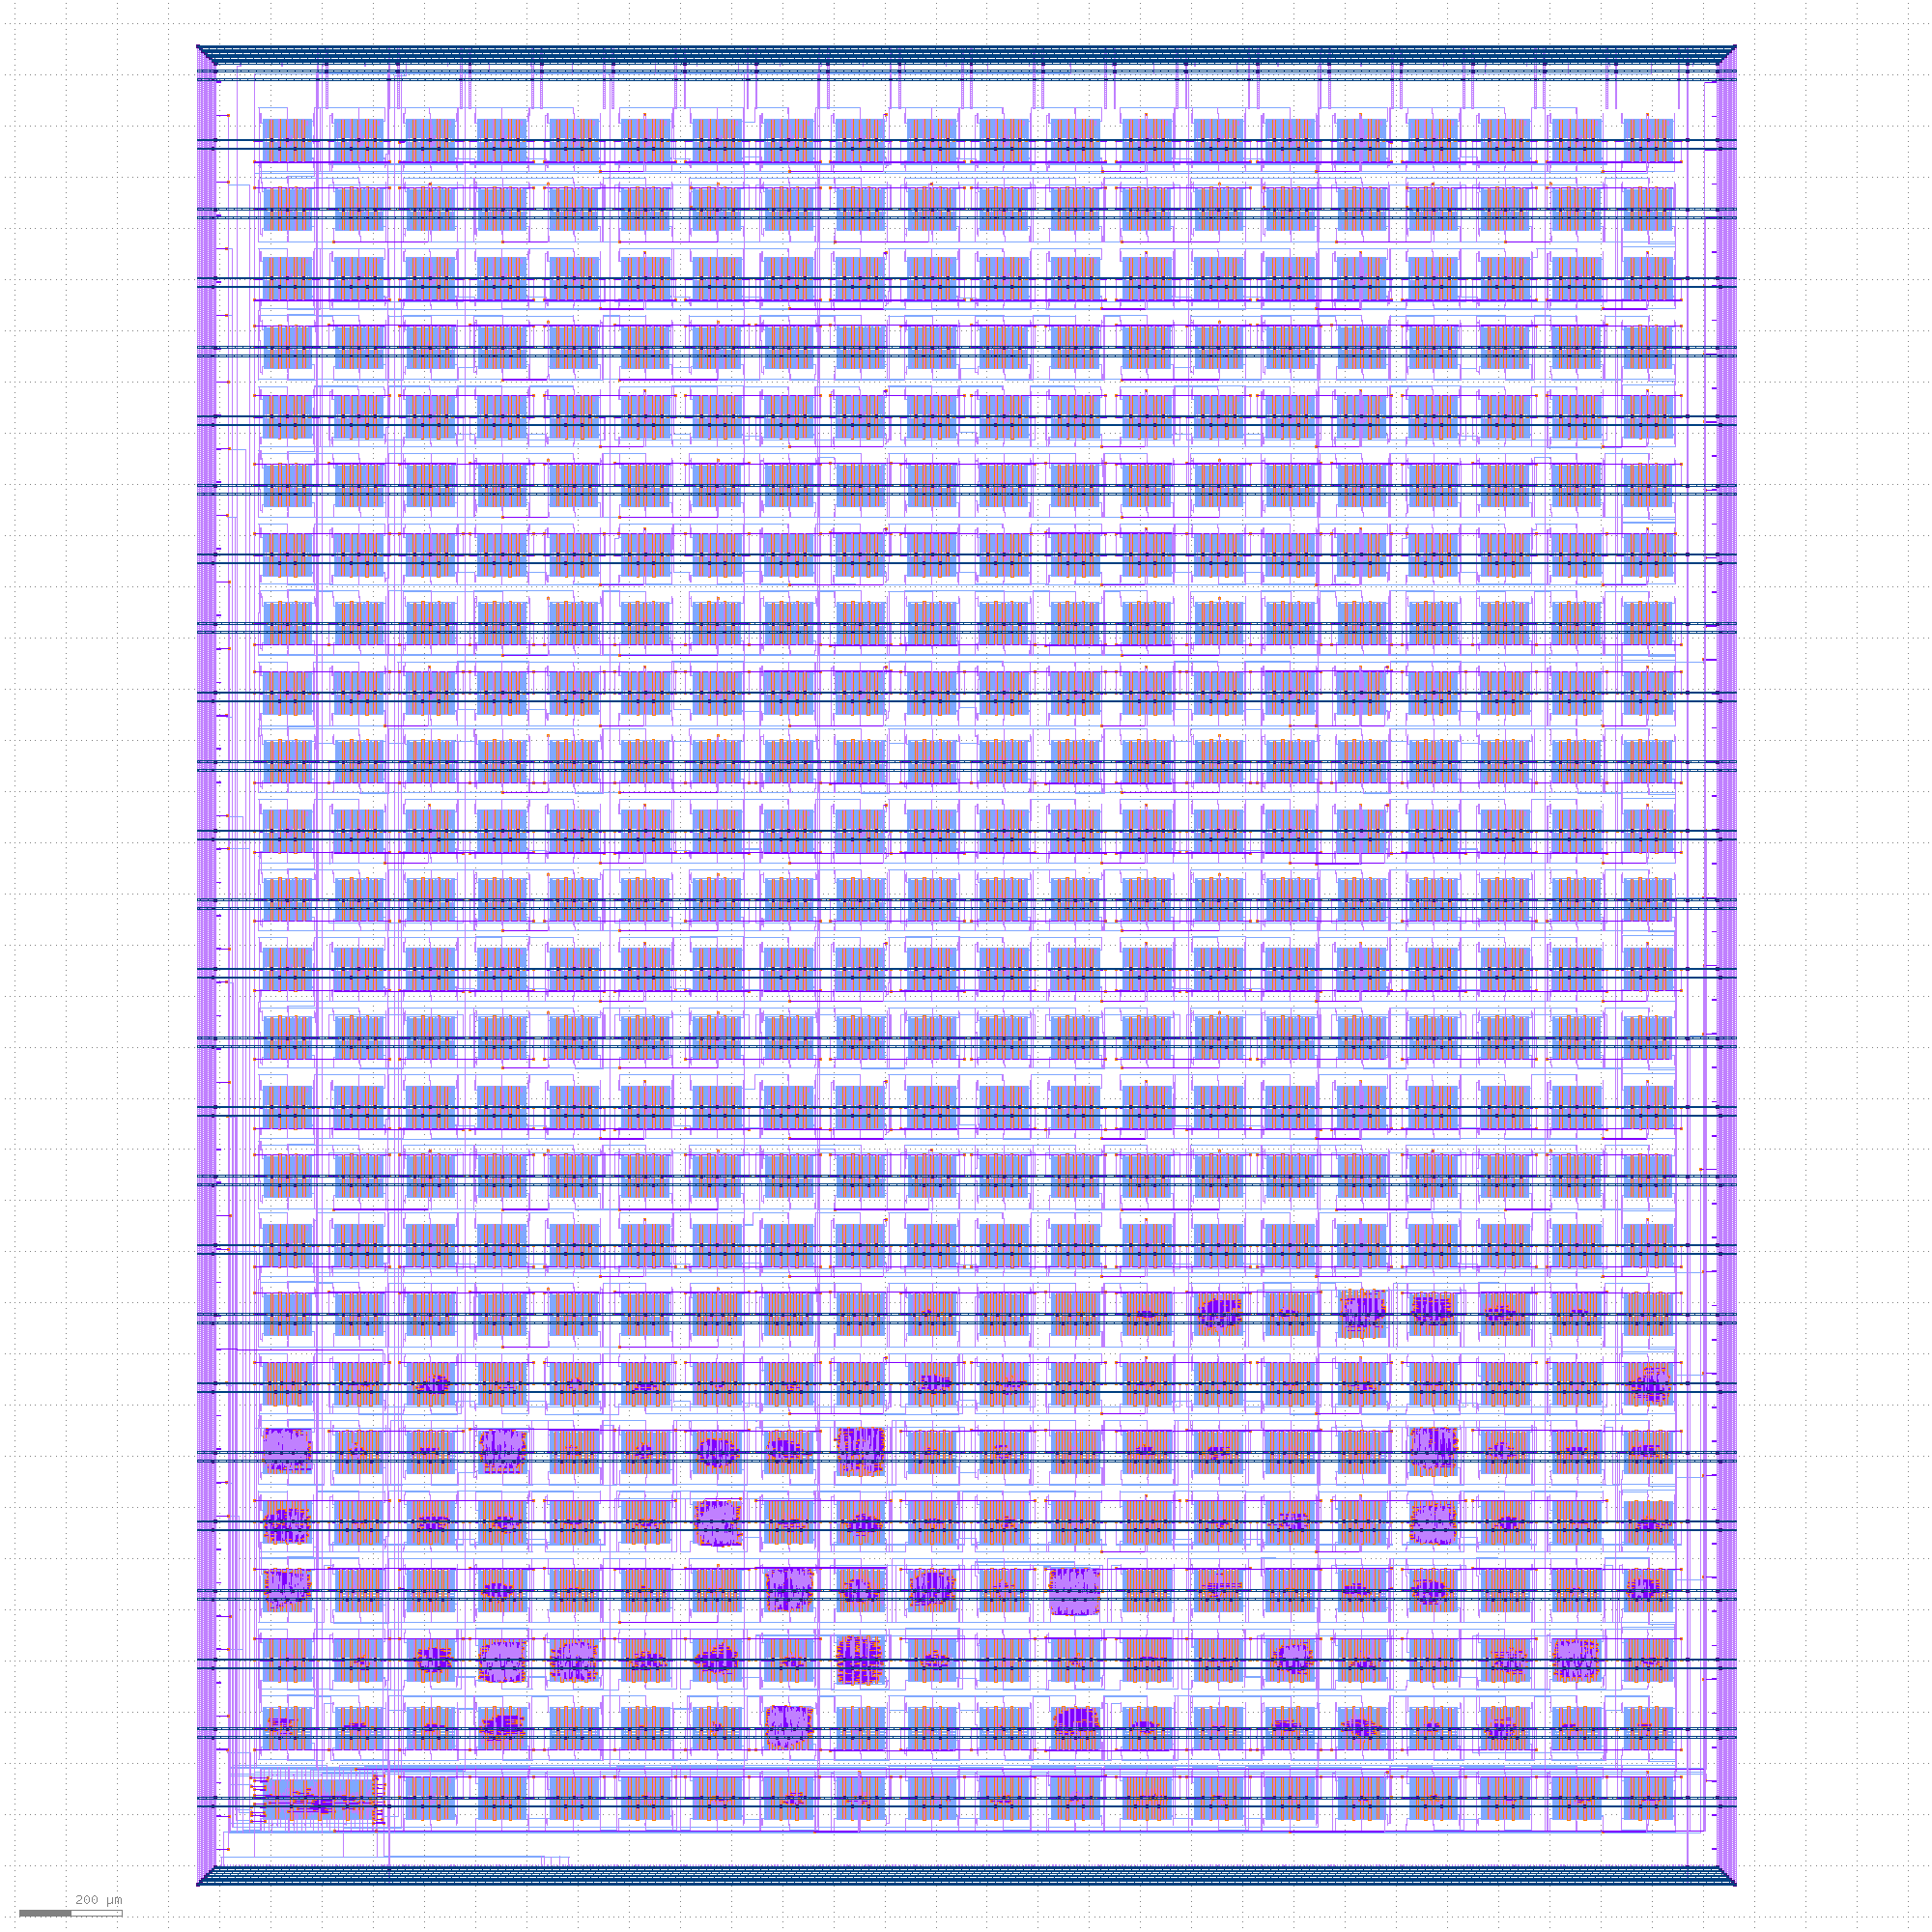
\includegraphics[width=1\columnwidth]{./Figs/tt01_whole_die.png}
\caption{500 designs connected in a chain for Tiny Tapeout 1; the scan chain driver can be seen in the lower left corner.}
\label{fig:500_designs_chain_TT01}
\end{figure}

\begin{figure}[!t]
\centering
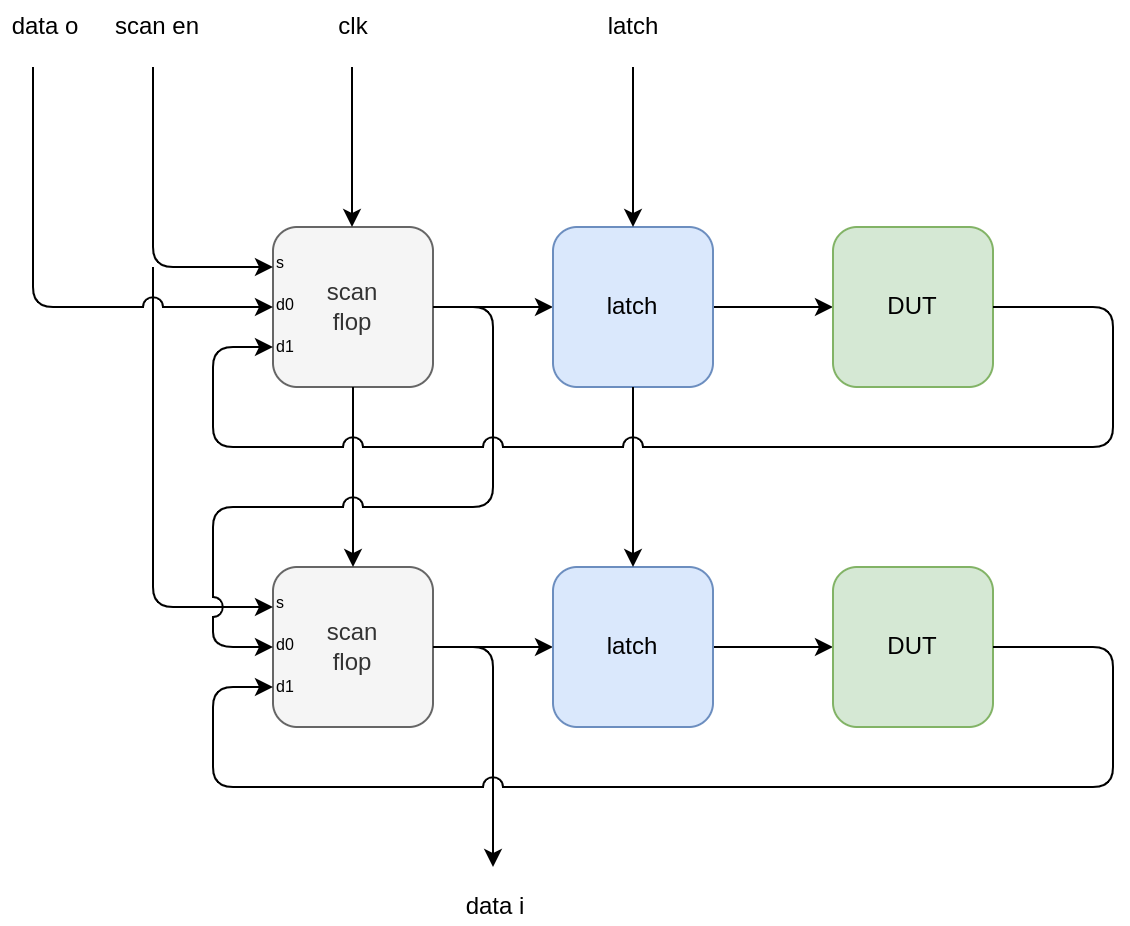
\includegraphics[width=\columnwidth]{./Figs/scanchain_block_diagram.png}
\caption{A simplified view of two Tiny Tapeout 1 designs in the scan chain.}
\label{fig:simplified_view_2_designs}
\end{figure}

Each design sends data into the secondary input of the scan flop and receives its own input from the output of the flop via a latch.
The chain is built~\cite{updateiodesign} by sending data from the output of the previous scan flop into the primary input of the next scan flop.
This arrangement allows the loading of data into any of the designs, followed by the capturing of the output and its clocking through the rest of the chain to the overall chain output.

While relatively easy to implement, a scan chain architecture has a downside: high latency.
As more designs are added to the chain it takes longer to send and receive data through it.
For example: assuming a \qty{50}{\MHz} scan chain clock with \qty{250} designs each having eight inputs and eight outputs, the maximum refresh rate of the resulting chain is $\qty{50}{\MHz} / (8 \times 250) = \qty{25}{\kHz}$.

The Tiny Tapeout 1 scan chain was embedded into each design, meaning a user could unintentionally remove it and break the chain.
This risk was mitigated with a formal equivalence check~\cite{tinytapeoutscan} which proves the chain was present in each submitted design and prevents submission if it has been removed.

Another concern with the scan chain design was hold violations, due to the large number of serially connected flops and potentially large clock skews over long signal wires. This was mitigated by reclocking the output data with a negative edge (negedge) flop, providing substantially more hold margin.

Following static timing analysis (STA) it was discovered that the clock duty cycle could change substantially due to the \qty{500} sequential clock drivers in the chain. Depending on the clock buffers and capacitance between each design the clock duty cycle could either increase or decrease, with this effect accumulated over the chain.

The verification effort~\cite{verificationmd} for the scan chain was broad and included a community review, register transfer level (RTL) and gate level (GL) simulation, formal verification\cite{sby}, STA, layout vs. schematic (LVS), DRC, and device level static verification~\cite{cvc}.
